\documentclass[12pt]{article}
\usepackage{fullpage}
\usepackage[colorlinks=true, urlcolor=blue, linkcolor=black]{hyperref}
\usepackage{graphicx}
\usepackage{float}
\usepackage{amsmath}
\usepackage{setspace}
\usepackage{sectsty}
\usepackage{fancyvrb}
\usepackage{mathtools}
\usepackage[flushleft]{threeparttable}

\begin{document}
\begin{center}
{\Large Applied Mathmamatics 221}\\
Project Milestone 2: Status Update\\
David Freed and Sam Green\\
\today
\end{center}

\section*{Overview of Main Progress}

We begin by addressing the questions 
described in the milestone description
and the return to more detailed discussion
after the overview. 

As it stands, we have not revised the goal
of our project, though we have introduced
an intermediate model building goal. The over
all goal of our project is still to assess
the relative strength of using time series
of tweets to build win probability models
relative to the the standard logistic
regression based predictive models that
currently in standard use. We have selected
a Hidden Markov based model as the end goal.
As a intermediate goal, however, we intend
to assess the basic predictve 
strength of the data by using the tweets
to predict the leader of the game at each
time period of the game. 

We have collected tweets for 35 
games, with a total of more than 500k so
far. This is more tweets per game than
the collected for previous studies. We
intend to collect data on the remaining
NCAA games next week. 

We address our previous stated goals below
in more detail, but broadly, we have
accomplished the majority of data collection
and have established a benchmark probability
model and have a good direction in which
to head towards our final deliverable. 

\section*{Status Update from Milestone 1}

We have reproduced the next steps that we made in the initial report below, with related commentary for each as to how much progress we have made on each. In sum, we have done almost all of the next steps that we proposed we would do earlier. 

\subsection*{Twitter Data Next Steps}
\subsubsection*{Get Twitter API keys}

\textit{This wasn't too hard.}

\subsubsection*{Identify the best way to get Twitter Data}

\textit{Did this.}

\subsubsection*{Read the literature on sensitivity analyses for Tweets}

\textit{This step has not yet been accomplished. It is a clear next step for the analysis that we will do in the immediate future, however.}

\subsubsection*{Get trial data}

\textit{Mostly done. We've successfully collected tweets
from 35 games from the NCAA March Madness
tournament, with a totally of about 500,000 tweets collected. The smallest pool for
one game that we've collected is 5,000,
and the smallest pool we've collected
is 50,000. This should allow
the dataset to be significant: previous
work used to analyze 768 games
in the NFL was based on an average of 
2,619 tweets per game. Our dataset has
on average 16,747 tweets per game so far. }

The data that we have collected has been
cleaned to include simply the tweet text
and a timestamp, though other axes of
information are available. We have so
far classified all of the tweets that
we have collected by game and created
infrastructure to build bucketed
time series of the tweets.

Initial analysis indicates that the data
we have collected should be adequate 
for the analysis we wish to perform 
(or at least isn't obviously inadequate).
Tweets are at reasonable volumes
through the collection period, with
notable spikes in volume likely
corresponding to game events. 
Pairing tweet timestamps to game timestamps
remains as a major next step (see next subsection), and see the linecharts below
for distributions of tweets for each game
we have collected. There's a broad
variety in the number of tweets collected,
since many games, especially in the early
rounds of tournament, took place at
the same time and between lower
visibility teams. Even the smallest
volumes have on the order of 100 tweets per minute.

\begin{figure} [H]
	\centering
	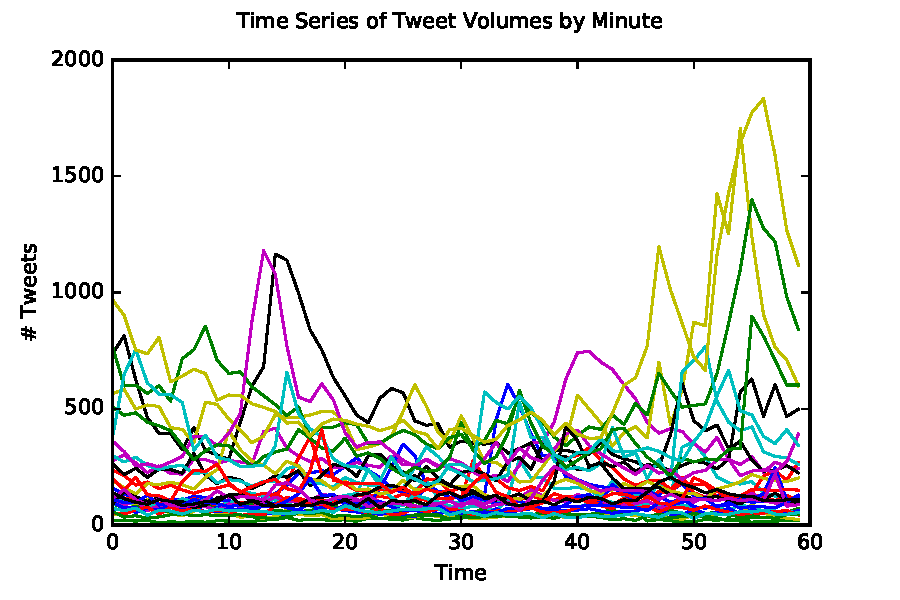
\includegraphics[scale = 0.7]{tweetvolues.pdf} 
	\caption{Example data taken from the Miami-Wichita State second round NCAA Tournament game}
\end{figure}

\subsection*{Box Score Data Next Steps}
\subsubsection*{Create a scraper to get all of the box score data}

The first thing that we did was to write a program that will scrape the box score data for any game. We took all data from \texttt{ESPN.com}, using the play-by-play data provided in the team pages (examples \href{http://espn.go.com/mens-college-basketball/playbyplay?gameId=400871280}{here}
 and \href{http://espn.go.com/mens-college-basketball/playbyplay?gameId=400871252}{here}
). Figure 1 below indicates what the data look like for every game.

\begin{figure} [H]
	\centering
	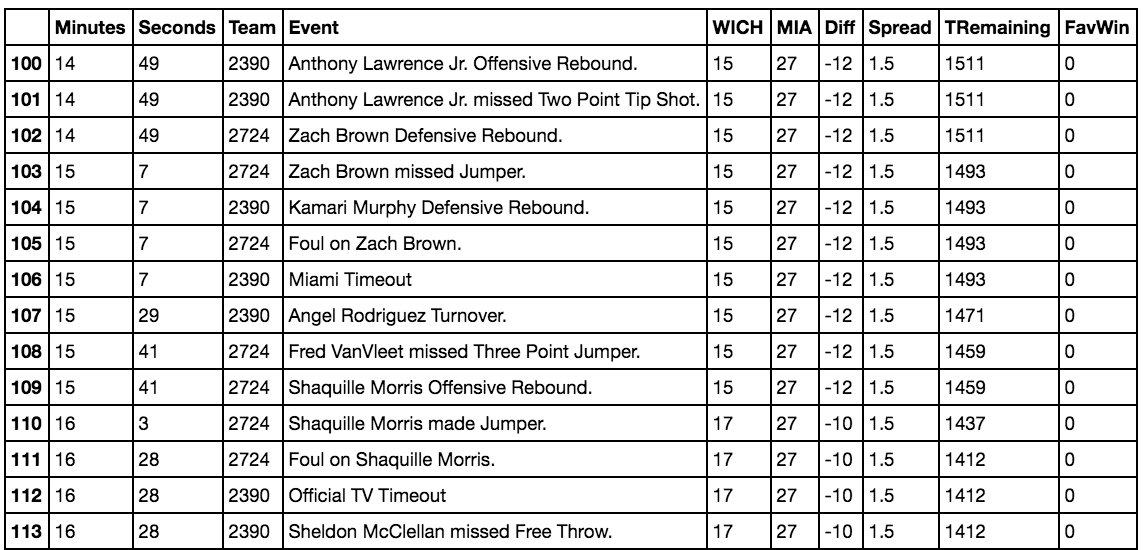
\includegraphics[scale = 0.7] {boxscore_data.png} 
	\caption{Example data taken from the Miami-Wichita State second round NCAA Tournament game}
\end{figure}

As we can say, not only do we know the time that has passed in every game, we also know the full event and the scores for each team at that point. We also have incorporated the point spread\footnote{For those readers unfamiliar with this concept, it refers to the consensus betting line put out from Vegas before the game. A team that is given a -2.5 point handicap is considered the favorite; any bettor who puts money on them will win if they win by three or more points. If the favorite loses, or wins by one or two points, he will lose his money. In the case that the team is favored by an integer (a line of -2 points, for example), if it wins by exactly that number, the house will return to the bettor the exact amount of money that he bet. This is referred to as a ``push" in standard gambling parlance.} from that game, the difference in the score after every play, and the eventual outcome (an indicator of whether the favorite won or not). 

While most of this data is not used until the following section, we did create functionality in our code\footnote{The above and below sections are all contained in the file \texttt{Box Score Scraper.ipynb}.} to generate game trend graphs for each game. An example trend graph for the Texas A\&M-Northern Iowa double-overtime game is shown below:

\begin{figure} [H]
	\centering
	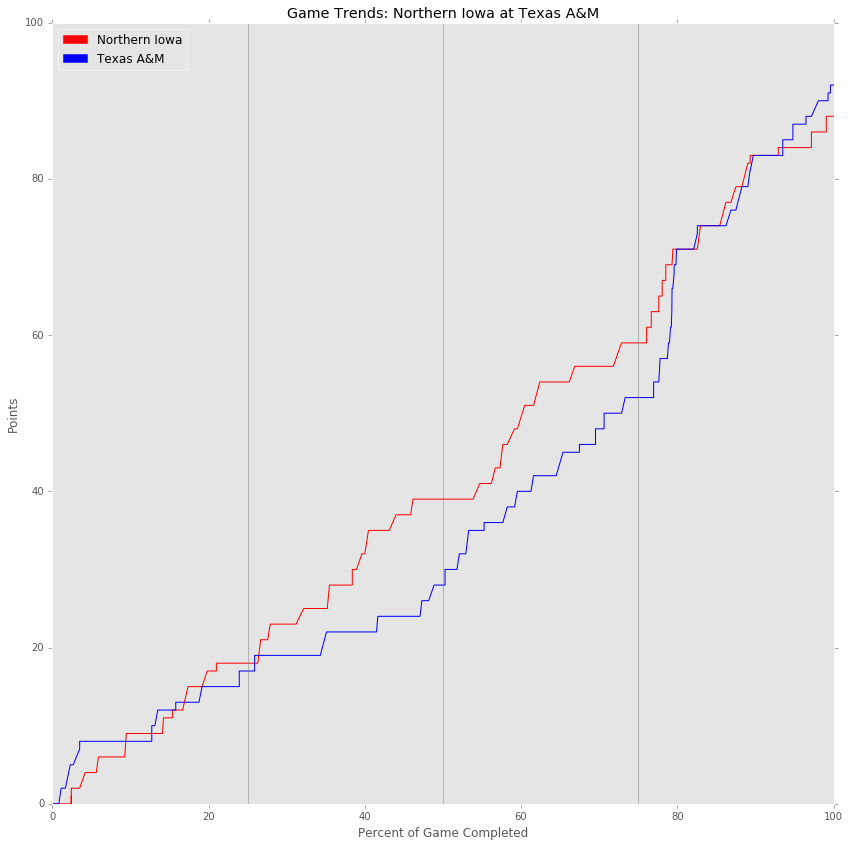
\includegraphics[scale = 0.3] {NI_TAMU.png} 
	\caption{Trend graph showing scores over time for the Texas A\&M-Northern Iowa second round NCAA Tournament game}
\end{figure}

\subsubsection*{Write a benchmark win probability model}

The next thing that we had to do was write a win probability model for the data. We did this by following the conventional research (see \href{http://fivethirtyeight.com/features/how-fivethirtyeight-is-forecasting-the-2016-ncaa-tournament/}{here} and \href{http://wagesofwins.com/2009/03/05/modeling-win-probability-for-a-college-basketball-game-a-guest-post-from-brian-burke/}{here}). The gist of the standard methodology is to collect a bunch of play-by-play data (of the type we have above) and then do a logistic regression in each time period based on the point spread and the difference in the game at that point in time.

We were able to implement this after some trouble, but did not fit the model to a lot of data. As of the writing of this document, we had just used a sample of 40 games to fit the data, which is much less than is typically used to fit the model (some versions that we have seen have used up to 20 times as many data). While the logistic regression model that we created predicted the final victor with about an 80 percent accuracy in each period (see table below), the coefficients varied so significantly across time periods that our win probability graphs were not nearly as smooth as we would like. 

\begin{table}[H] 
\centering  
\caption{Model's probability of predicting the winner correctly}   
\begin{tabular}{c c}
\hline \hline
Minutes Remaining & Odds of Correctly Predicting Victory \\ [0.5ex]
\hline
0 & 0.8925 \\
5 & 0.8577 \\
10 & 0.7964 \\
15 & 0.7542 \\
20 & 0.7899 \\ 
25 & 0.8178 \\ 
30 & 0.7706 \\ 
35 & 0.6946 \\ 
40 & 0.7934 \\
\hline
\end{tabular}
\end{table}

Given that we have directly replicated prior analysis, however, we aim just to fit the model to more data in the future. We do not anticipate any conceptual, only logistical, difficulties in assembling this data; however, given the time and thesis constraints of this deadline, we sadly were not able to do so early. 

\section*{Next Steps}

Our project proposal demanded that we have three major items in order to run the tests we wanted:
\begin{enumerate}
	\item \textbf{Game-by-game Twitter data}. As described above, we need this to be able to gauge fan sentiment at every point during the game so that we can get their impression on how the game is going
	\item \textbf{Game progress data}. This comprises both the score at each point in time\footnote{Of more importance to us is the difference in scores---whether a team is up 100-90 or 10-0 is immaterial; the ex ante predictors of team strength we used are based in the predicted final score difference.} and the probability of the favorite winning at each point in time
	\item \textbf{Twitter prediction model}. For our final results, we will essentially be comparing the standard win probability models above to the Twitter prediction model that we build. Sentiment analysis also remains to be accomplished, but requires a repurposing of
	existing infrastructure. 
\end{enumerate}

Consequently, we can say that we have accomplished most of our goals. While there are minor things to do on the first two points\footnote{One thing that jumps out as an immediate next step on the data is matching analog times (i.e. 2:00 EST) from the Tweets to the time left in the game. This will allow us to directly match the predictions by Twitter to predictions made by the win probability model.} we are mostly focused now on creating the Twitter model. 

To accomplish that, we will need to know how to classify the Tweets by strength of sentiment. Our task after that is to think about how to map those sensitivity analyses to a point spread. Once we do that, we can test our model against basic default models of win probability and see how well Twitter performs, which will give us the desired final results.  

\end{document}